\begin{figure}[tbp]
\centering
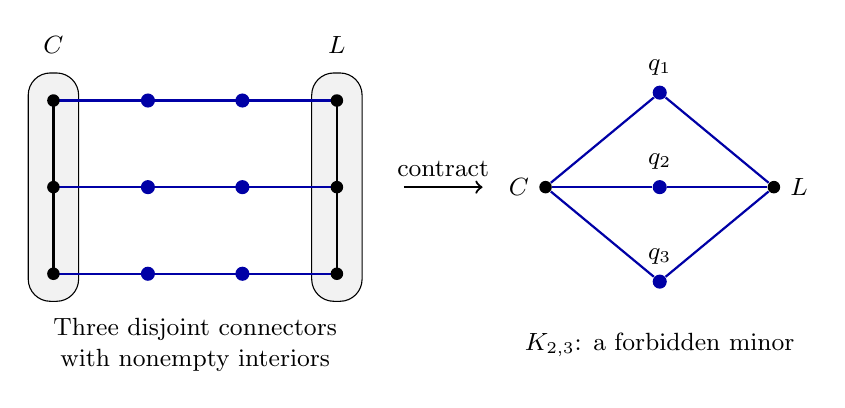
\begin{tikzpicture}[x=1cm,y=1cm,font=\small,
  vertex/.style={circle,fill=black,inner sep=1.6pt},
  interior/.style={circle,fill=blue!65!black,inner sep=1.8pt}]
  \draw[fill=gray!10,rounded corners=8pt] (-.32,-1.45) rectangle (.32,1.45);
  \draw[fill=gray!10,rounded corners=8pt] (3.28,-1.45) rectangle (3.92,1.45);
  \draw[thick] (0,-1.1)--(0,1.1);
  \draw[thick] (3.6,-1.1)--(3.6,1.1);
  \foreach \y in {-1.1,0,1.1} {
    \draw[blue!65!black,thick] (0,\y)--(3.6,\y);
    \node[vertex] at (0,\y) {};
    \node[vertex] at (3.6,\y) {};
    \node[interior] at (1.2,\y) {};
    \node[interior] at (2.4,\y) {};
  }
  \node at (0,1.8) {$C$};
  \node at (3.6,1.8) {$L$};
  \node[align=center] at (1.8,-2) {Three disjoint connectors\\with nonempty interiors};
  \draw[->,thick] (4.45,0)--(5.45,0) node[midway,above] {contract};

  \node[vertex,label=left:$C$] (C) at (6.25,0) {};
  \node[vertex,label=right:$L$] (L) at (9.15,0) {};
  \foreach \y/\k in {1.2/1,0/2,-1.2/3} {
    \node[interior,label=above:$q_\k$] (q\k) at (7.7,\y) {};
    \draw[blue!65!black,thick] (C)--(q\k)--(L);
  }
  \node at (7.7,-2) {$K_{2,3}$: a forbidden minor};
\end{tikzpicture}
\caption{The hypothetical obstruction in Lemma~\ref{geo:portals}.
Three sufficiently separated entrance points would give vertex-disjoint
paths from the connected high set $C$ to the connected low set $L$.
After trimming, each connector has a nonempty interior avoiding both
sets. Contracting $C$, $L$, and the three interiors gives $K_{2,3}$,
which cannot be a minor of the outerplanar column graph.
The drawing records this contraction; it is not an outerplanar drawing
of a configuration that the column model permits.}
\label{fig:two-portals}
\end{figure}
